

% Options for packages loaded elsewhere
\PassOptionsToPackage{unicode}{hyperref}
\PassOptionsToPackage{hyphens}{url}
%
\documentclass[
  man]{apa6}
\usepackage{lmodern}
\usepackage{amssymb,amsmath}
\usepackage{ifxetex,ifluatex}
\ifnum 0\ifxetex 1\fi\ifluatex 1\fi=0 % if pdftex
  \usepackage[T1]{fontenc}
  \usepackage[utf8]{inputenc}
  \usepackage{textcomp} % provide euro and other symbols
\else % if luatex or xetex
  \usepackage{unicode-math}
  \defaultfontfeatures{Scale=MatchLowercase}
  \defaultfontfeatures[\rmfamily]{Ligatures=TeX,Scale=1}
\fi
% Use upquote if available, for straight quotes in verbatim environments
\IfFileExists{upquote.sty}{\usepackage{upquote}}{}
\IfFileExists{microtype.sty}{% use microtype if available
  \usepackage[]{microtype}
  \UseMicrotypeSet[protrusion]{basicmath} % disable protrusion for tt fonts
}{}
\makeatletter
\@ifundefined{KOMAClassName}{% if non-KOMA class
  \IfFileExists{parskip.sty}{%
    \usepackage{parskip}
  }{% else
    \setlength{\parindent}{0pt}
    \setlength{\parskip}{6pt plus 2pt minus 1pt}}
}{% if KOMA class
  \KOMAoptions{parskip=half}}
\makeatother
\usepackage{xcolor}
\IfFileExists{xurl.sty}{\usepackage{xurl}}{} % add URL line breaks if available
\IfFileExists{bookmark.sty}{\usepackage{bookmark}}{\usepackage{hyperref}}
\hypersetup{
  pdftitle={Correlations between the sample means difference and standardizers of all estimators, and implications on biases and variances of all estimators},
  pdfauthor={Delacre Marie},
  pdfkeywords={keywords},
  hidelinks,
  pdfcreator={LaTeX via pandoc}}
\urlstyle{same} % disable monospaced font for URLs
\usepackage{longtable,booktabs}
% Correct order of tables after \paragraph or \subparagraph
\usepackage{etoolbox}
\makeatletter
\patchcmd\longtable{\par}{\if@noskipsec\mbox{}\fi\par}{}{}
\makeatother
% Allow footnotes in longtable head/foot
\IfFileExists{footnotehyper.sty}{\usepackage{footnotehyper}}{\usepackage{footnote}}
\makesavenoteenv{longtable}
\usepackage{graphicx,grffile}
\makeatletter
\def\maxwidth{\ifdim\Gin@nat@width>\linewidth\linewidth\else\Gin@nat@width\fi}
\def\maxheight{\ifdim\Gin@nat@height>\textheight\textheight\else\Gin@nat@height\fi}
\makeatother
% Scale images if necessary, so that they will not overflow the page
% margins by default, and it is still possible to overwrite the defaults
% using explicit options in \includegraphics[width, height, ...]{}
\setkeys{Gin}{width=\maxwidth,height=\maxheight,keepaspectratio}
% Set default figure placement to htbp
\makeatletter
\def\fps@figure{htbp}
\makeatother
\setlength{\emergencystretch}{3em} % prevent overfull lines
\providecommand{\tightlist}{%
  \setlength{\itemsep}{0pt}\setlength{\parskip}{0pt}}
\setcounter{secnumdepth}{-\maxdimen} % remove section numbering
\shorttitle{}
\affiliation{
\vspace{0.5cm}
\textsuperscript{1} ULB}
\keywords{keywords\newline\indent Word count: X}
\usepackage{csquotes}
\usepackage{upgreek}
\captionsetup{font=singlespacing,justification=justified}

\usepackage{longtable}
\usepackage{lscape}
\usepackage{multirow}
\usepackage{tabularx}
\usepackage[flushleft]{threeparttable}
\usepackage{threeparttablex}

\newenvironment{lltable}{\begin{landscape}\begin{center}\begin{ThreePartTable}}{\end{ThreePartTable}\end{center}\end{landscape}}

\makeatletter
\newcommand\LastLTentrywidth{1em}
\newlength\longtablewidth
\setlength{\longtablewidth}{1in}
\newcommand{\getlongtablewidth}{\begingroup \ifcsname LT@\roman{LT@tables}\endcsname \global\longtablewidth=0pt \renewcommand{\LT@entry}[2]{\global\advance\longtablewidth by ##2\relax\gdef\LastLTentrywidth{##2}}\@nameuse{LT@\roman{LT@tables}} \fi \endgroup}


\DeclareDelayedFloatFlavor{ThreePartTable}{table}
\DeclareDelayedFloatFlavor{lltable}{table}
\DeclareDelayedFloatFlavor*{longtable}{table}
\makeatletter
\renewcommand{\efloat@iwrite}[1]{\immediate\expandafter\protected@write\csname efloat@post#1\endcsname{}}
\makeatother
\usepackage{lineno}

\linenumbers

\title{Correlations between the sample means difference and standardizers of all estimators, and implications on biases and variances of all estimators}
\author{Delacre Marie\textsuperscript{1}}
\date{}

\begin{document}
\maketitle

\hypertarget{introduction}{%
\section{Introduction}\label{introduction}}

The \emph{d}-family effect sizes are commonly used with \enquote{between-subject} designs where individuals are randomly assigned into one of two independent groups and groups scores means are compared. The population effect size is defined as

\begin{equation} 
\delta = \frac{\mu_{1}-\mu_{2}}{\sigma} 
\label{eq:Cohendelta}
\end{equation}

where both populations follow a normal distribution with mean \(\mu_j\) in the \(j^{th}\) population (j=1,2) and common standard deviation \(\sigma\). They exist different estimators of this population effect size, varying as a function of the chosen standardizer (\(\sigma\)). When the equality of variances assumption is met, \(\sigma\) is estimated by pooling both samples standard deviations (\(S_1\) and \(S_2\)):

\begin{equation} 
\sigma_{Cohen's \; d_s} = \sqrt{\frac{(n_1-1) \times S_1^2+(n_2-1) \times S_2^2}{n_1+n_2-2}}
\label{eq:Cohends}
\end{equation}

When the equality of variances assumption is not met, we are considering three alternative estimates:

\begin{itemize}
\tightlist
\item
  Using the standard deviation of the control group (\(S_c\)) as standardizer:
\end{itemize}

\begin{equation} 
S_{Glass's \; d_s} = S_{c}
\label{eq:Glassds}
\end{equation}

\begin{itemize}
\tightlist
\item
  Using a standardizer that takes the sample sizes allocation ratio \(\left( \frac{n_1}{n_2}\right)\) into account:
\end{itemize}

\begin{equation} 
S_{Shieh's \; d_s} = \sqrt{S_1^2/q_1+S_2^2/q_2}; \;\;\; q_j=\frac{n_j}{N} (j=1,2)
\label{eq:Shiehds}
\end{equation}

\begin{itemize}
\tightlist
\item
  Or using the square root of the non pooled average of both variance estimates (\(S^2_1\) and \(S^2_2\)) as standardizer:
\end{itemize}

\begin{equation} 
S_{Cohen's \; d'_s} = \sqrt{\frac{\left(S^2_{1}+S^2_{2} \right)}{2}}
\label{eq:cohenprimeds}
\end{equation}

As we previously mentioned, using these formulas implies meeting the assumption of normality. Using them when distributions are not normal will have consequences on both bias and variance of all estimators. More specifically, when samples are extracted from skewed distribution, correlations might occur between the sample means difference (\(\bar{X_1}-\bar{X_2}\)) and standardizers (\(\sigma\)). Studying when these correlations occur is the main goal of this appendix. To this end, we will distinguish 4 situations, as a function of the sample sizes ratio \(\left( \frac{n_1}{n_2}=1 \; vs. \frac{n_1}{n_2}\neq1\; \right)\) and the population \(SD\)-ratio \(\left( \frac{\sigma_1}{\sigma_2}=1 \; vs. \frac{\sigma_1}{\sigma_2}\neq1\; \right)\), but before that, we will briefly introduce the impact of correlations on the bias.

Note that we will compute correlations using the coefficient of Spearman's \(\rho\). We decided to use Spearman's \(\rho\) instead of Pearson's \(\rho\) because some plots revealed non-perfectly linear relations.

\hypertarget{how-correlations-between-the-mean-difference-barx_1-barx_2-and-standardizers-affect-the-bias-of-estimators.}{%
\section{\texorpdfstring{How correlations between the mean difference (\(\bar{X_1}-\bar{X_2}\)) and standardizers affect the bias of estimators.}{How correlations between the mean difference (\textbackslash bar\{X\_1\}-\textbackslash bar\{X\_2\}) and standardizers affect the bias of estimators.}}\label{how-correlations-between-the-mean-difference-barx_1-barx_2-and-standardizers-affect-the-bias-of-estimators.}}

When distributions are right-skewed, there is a positive (negative) correlation between \(S_1\) (\(S_2\)) and (\(\bar{X_1}-\bar{X_2}\)). When distributions are left-skewed, there is a negative (positive) correlation between \(S_1\) (\(S_2\)) and \(\bar{X_1}-\bar{X_2}\). When the population mean difference \(\mu_1-\mu_2\) is positive (like in our simulations), all other parameters being equal, an estimator is always less biased and variable when choosing a standardizer that is positively correlated with \(\bar{X_1}-\bar{X_2}\) than when choosing an estimator that is negatively correlated with \(\bar{X_1}-\bar{X_2}\). When the population mean difference is negative, the reverse is true.

GRAPHIQUE POUR L'EXPLIQUER.

Note: I mentioned \enquote{all other parameters being equal}, because it is always possible that other factors in action have an opposite effect on bias and variance in order that increasing the magnitude of the correlation between \(S_j\) and \(\bar{X_1}-\bar{X_2}\) does not necessarily reduce the bias and the variance. For example, when population variances are equal across groups and sample sizes are unequal, we will see below that the lower \(n_j\), the larger the magnitude of the correlation between \(S_j\) and \(\bar{X_1}-\bar{X_2}\). When the correlation between \(S_j\) and \(\bar{X_1}-\bar{X_2}\) is positive, the smaller the sample size, the larger the positive correlation. At the same time, we know that increasing the sample size decrease the bias. This is a nice example of situations where two factors might have an opposite action on bias.

\hypertarget{correlations-between-the-mean-difference-barx_1-barx_2-and-all-standardizers}{%
\section{\texorpdfstring{Correlations between the mean difference (\(\bar{X_1}-\bar{X_2}\)) and all standardizers}{Correlations between the mean difference (\textbackslash bar\{X\_1\}-\textbackslash bar\{X\_2\}) and all standardizers}}\label{correlations-between-the-mean-difference-barx_1-barx_2-and-all-standardizers}}

\hypertarget{when-equal-population-variances-are-estimated-based-on-equal-sample-sizes-condition-a}{%
\subsection{When equal population variances are estimated based on equal sample sizes (condition a)}\label{when-equal-population-variances-are-estimated-based-on-equal-sample-sizes-condition-a}}

\begin{figure}
\centering
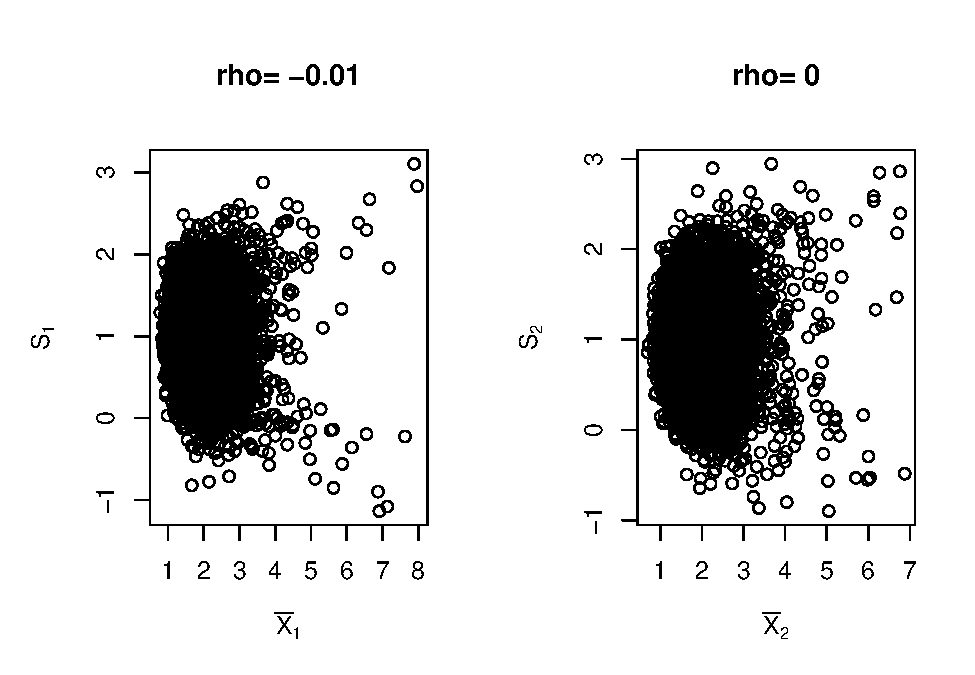
\includegraphics{Correlations-between-the-sample-means-difference-and-standardizers-of-all-estimators,-and-implications-on-biases-and-variances-of-all-estimators_files/figure-latex/C1sym-1.pdf}
\caption{\label{fig:C1sym}\(S_j\) as a function of \(\bar{X_j}\) (j=1,2), when samples are extracted from symmetric distributions (\(\gamma_1 = 0\))}
\end{figure}

While \(\bar{X_j}\) and \(S_j\) (j=1,2) are uncorrelated when samples are extracted from symmetric distributions (see Figure \ref{fig:C1sym}), there is a non-null correlation between \(\bar{X_j}\) and \(S_j\) when distributions are skewed (Zhang, 2007).

\begin{figure}
\centering
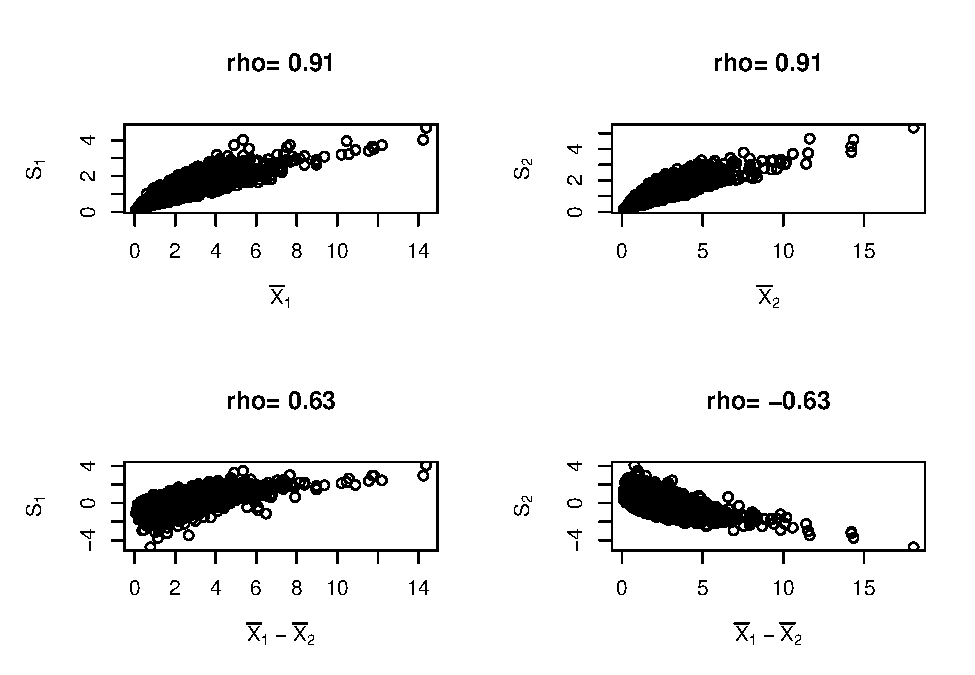
\includegraphics{Correlations-between-the-sample-means-difference-and-standardizers-of-all-estimators,-and-implications-on-biases-and-variances-of-all-estimators_files/figure-latex/SDC1Rs-1.pdf}
\caption{\label{fig:SDC1Rs}\(S_j\) (j=1,2) as a function \(\bar{X_j}\) (top plots) or \(\bar{X_1}-\bar{X_2}\) (bottom plots), when samples are extracted from right skewed distributions (\(\gamma_1 = 6.32\); top plots)}
\end{figure}

More specifically, when distributions are right-skewed, there is a \textbf{positive} correlation between \(\bar{X_j}\) and \(S_j\) (see the two top plots in Figure \ref{fig:SDC1Rs}), resulting in a \emph{positive} correlation between \(S_1\) and \(\bar{X_1}-\bar{X_2}\) and in a \emph{negative} correlation between \(S_2\) and \(\bar{X_1}-\bar{X_2}\) (see the two bottom plots in Figure \ref{fig:SDC1Rs}). This can be explained by the fact that \(\bar{X_1}\) and \(\bar{X_1}-\bar{X_2}\) are positively correlated while \(\bar{X_2}\) and \(\bar{X_1}-\bar{X_2}\) and negatively correlated (of course, correlations would be trivially reversed if we computed \(\bar{X_2}-\bar{X_1}\) instead of \(\bar{X_1}-\bar{X_2}\)).

\begin{figure}
\centering
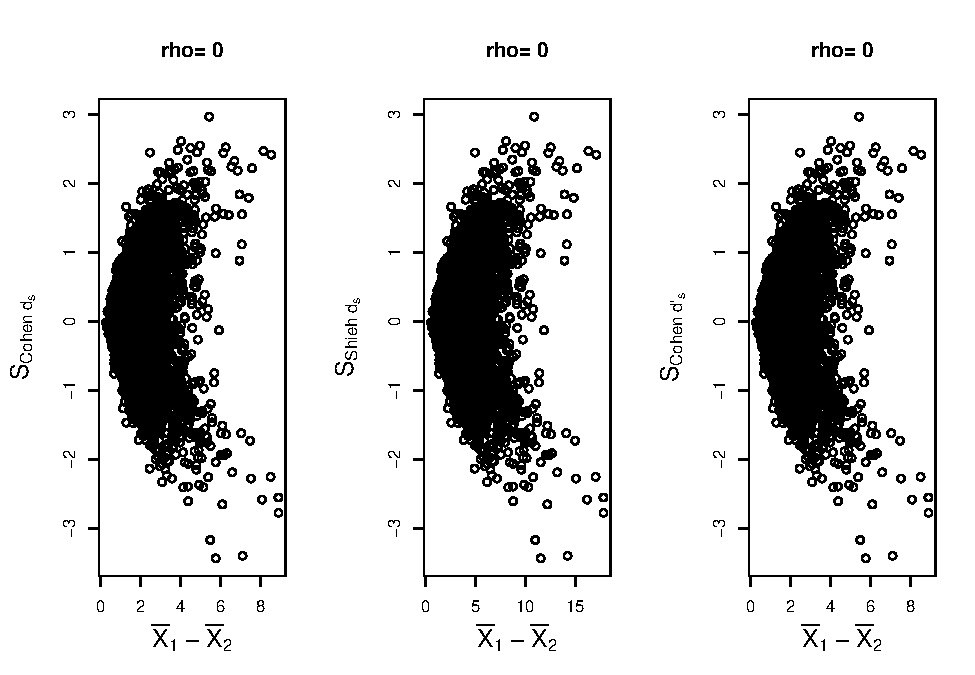
\includegraphics{Correlations-between-the-sample-means-difference-and-standardizers-of-all-estimators,-and-implications-on-biases-and-variances-of-all-estimators_files/figure-latex/StdzrC1Rs-1.pdf}
\caption{\label{fig:StdzrC1Rs}\(S_{Glass's \; d_s}\), \(S_{Shieh's \; d_s}\) and \(S_{Cohen's \; d'_s}\) as a function of the means difference (\(\bar{X_1}-\bar{X_2}\)), when samples are extracted from right skewed distributions (\(\gamma_1 = 6.32\))}
\end{figure}

One should also notice that both correlations between \(S_j\) and \(\bar{X_1}-\bar{X_2}\) are equal, in absolute terms (possible tiny differences might be observed due to sampling error in our simulations). As a consequence, when computing a standardizer taking both \(S_1\) and \(S_2\) into account, it results in a standardizer that is uncorrelated with \(\bar{X_1}-\bar{X_2}\) (see Figure \ref{fig:StdzrC1Rs}).

\begin{figure}
\centering
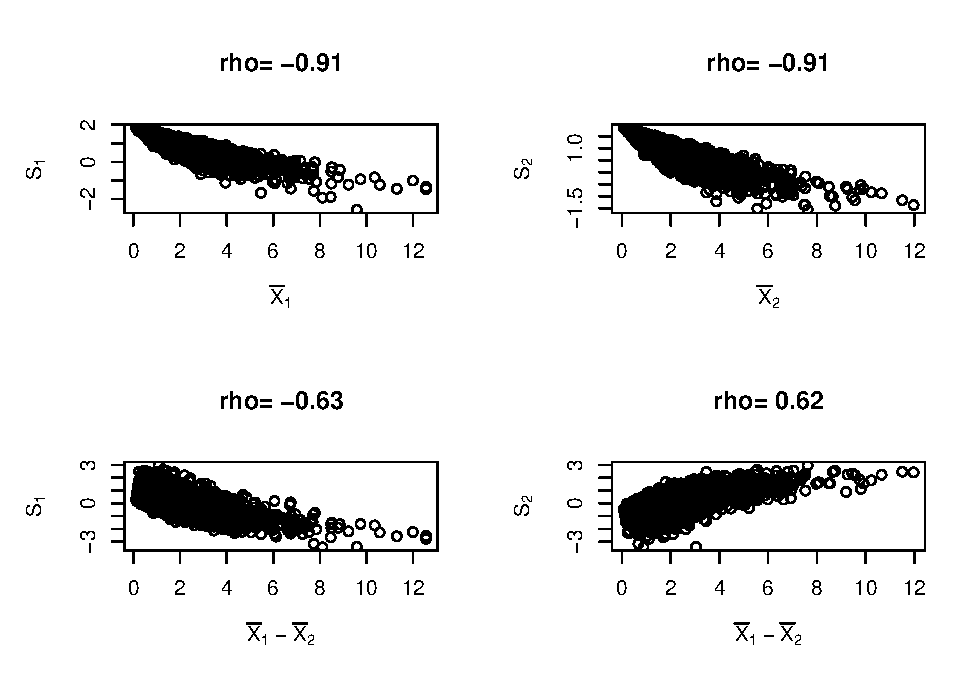
\includegraphics{Correlations-between-the-sample-means-difference-and-standardizers-of-all-estimators,-and-implications-on-biases-and-variances-of-all-estimators_files/figure-latex/SDC1Ls-1.pdf}
\caption{\label{fig:SDC1Ls}\(S_j\) (j=1,2) as a function \(\bar{X_j}\) (top plots) or \(\bar{X_1}-\bar{X_2}\) (bottom plots), when samples are extracted from left skewed distributions (\(\gamma_1 = -6.32\); top plots)}
\end{figure}

On the other hand, when distributions are left-skewed, there is a \textbf{negative} correlation between \(\bar{X_j}\) and \(S_j\) (see the two top plots in Figure \ref{fig:SDC1Ls}), resulting in a \emph{negative} correlation between \(S_1\) and \(\bar{X_1}-\bar{X_2}\) and in a \emph{positive} correlation between \(S_2\) and \(\bar{X_1}-\bar{X_2}\) (see the two bottom plots in Figure \ref{fig:SDC1Ls}).

\begin{figure}
\centering
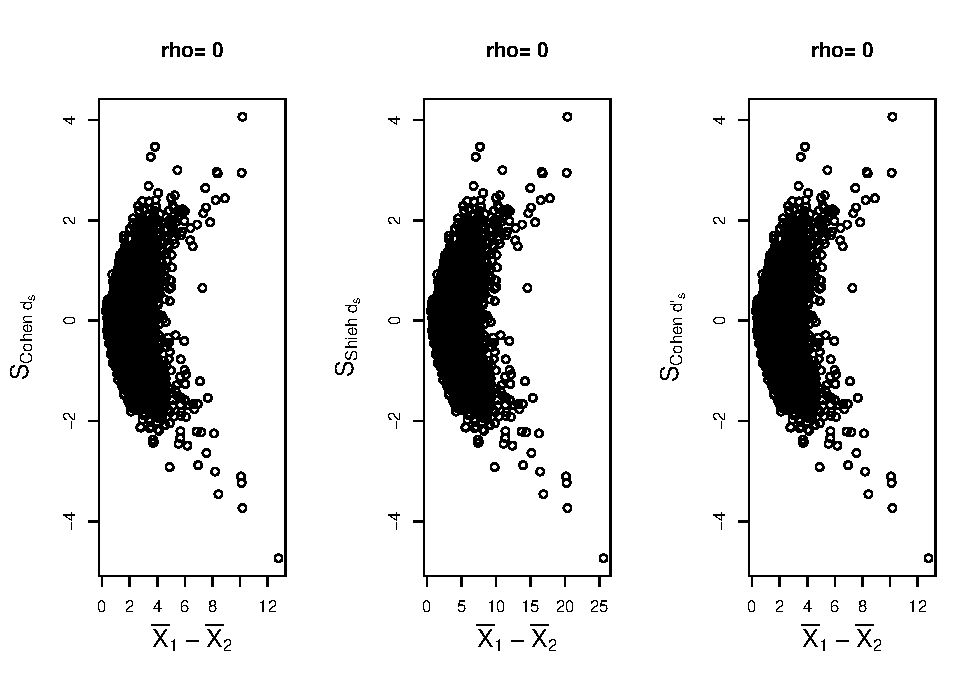
\includegraphics{Correlations-between-the-sample-means-difference-and-standardizers-of-all-estimators,-and-implications-on-biases-and-variances-of-all-estimators_files/figure-latex/StdzrC1Ls-1.pdf}
\caption{\label{fig:StdzrC1Ls}\(S_{Glass's \; d_s}\), \(S_{Shieh's \; d_s}\) and \(S_{Cohen's \; d'_s}\) as a function of the means difference (\(\bar{X_1}-\bar{X_2}\)), when samples are extracted from left skewed distributions (\(\gamma_1 = -6.32\))}
\end{figure}

Again, because correlations between \(S_j\) and \(\bar{X_1}-\bar{X_2}\) are similar in absolute terms, any standardizers taking both \(S_1\) and \(S_2\) into account will be uncorrelated with \(\bar{X_1}-\bar{X_2}\) (see Figure \ref{fig:StdzrC1Ls}).

\hypertarget{when-equal-population-variances-are-estimated-based-on-unequal-sample-sizes-condition-b}{%
\subsection{When equal population variances are estimated based on unequal sample sizes (condition b)}\label{when-equal-population-variances-are-estimated-based-on-unequal-sample-sizes-condition-b}}

When distributions are skewed, there are again non-null correlations between \(\bar{X_j}\) and \(S_j\), however \(cor(S_1,\bar{X_1}) \neq cor(S_2,\bar{X_2})\), because of the different sample sizes.

\begin{figure}
\centering
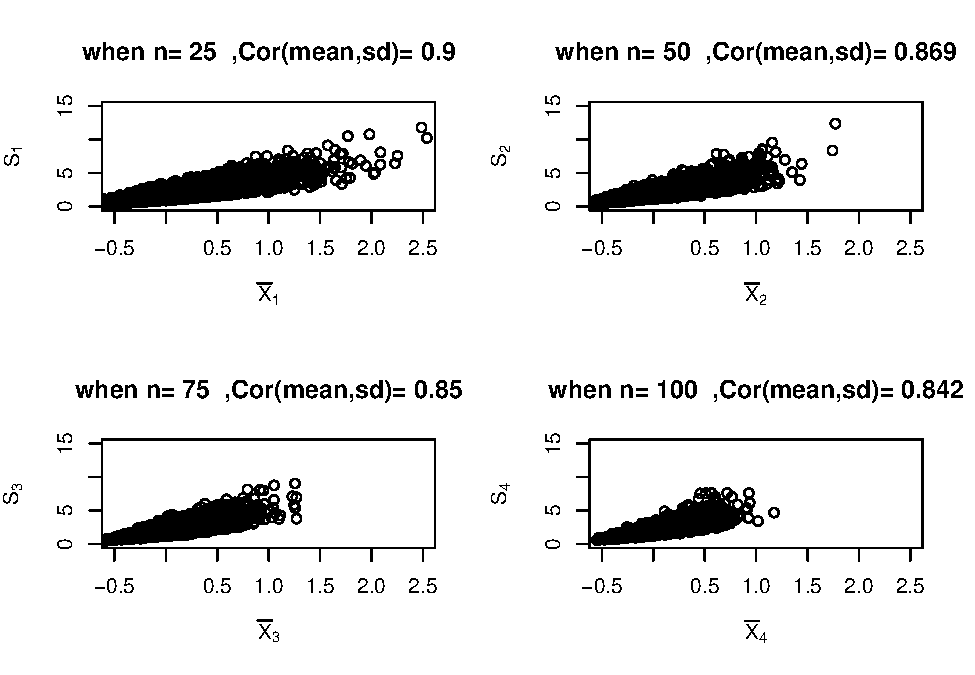
\includegraphics{Correlations-between-the-sample-means-difference-and-standardizers-of-all-estimators,-and-implications-on-biases-and-variances-of-all-estimators_files/figure-latex/C2corn-1.pdf}
\caption{\label{fig:C2corn}correlation between \(S_j\) and \(\bar{X_j}\) when n = 25, 50, 75 or 100 and samples are extracted from right skewed distributions (\(\gamma_1 = 6.32\))}
\end{figure}

\begin{figure}
\centering
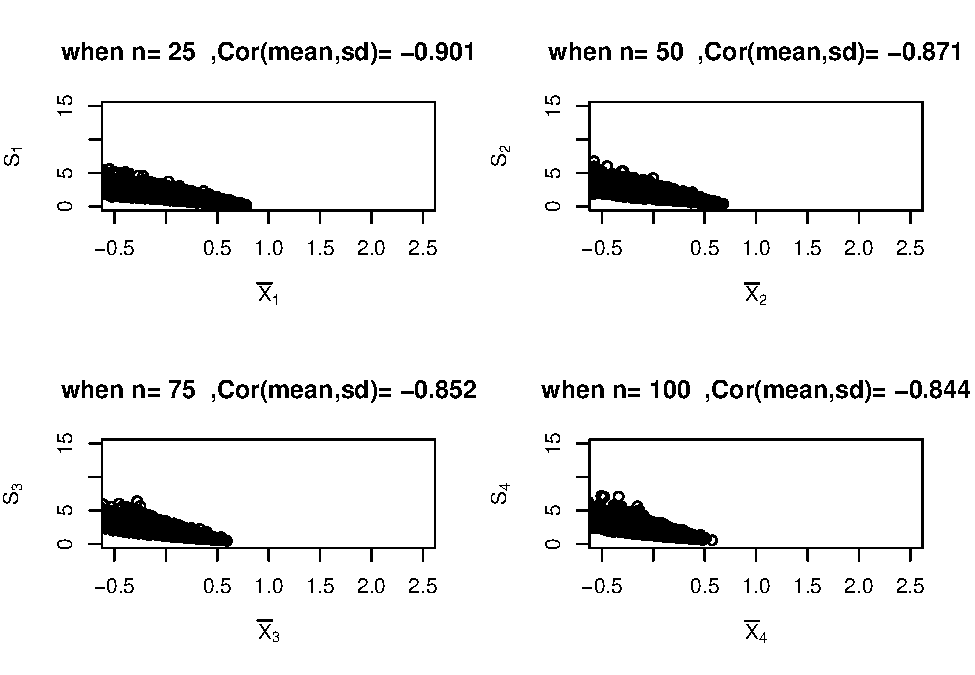
\includegraphics{Correlations-between-the-sample-means-difference-and-standardizers-of-all-estimators,-and-implications-on-biases-and-variances-of-all-estimators_files/figure-latex/C2corn2-1.pdf}
\caption{\label{fig:C2corn2}correlation between \(S_j\) and \(\bar{X_j}\) when n = 25, 50, 75 or 100 and samples are extracted from right left distributions (\(\gamma_1 = -6.32\))}
\end{figure}

When distributions are skewed, one observes that the larger the sample size, the lower the correlation between \(S_j\) and \(\bar{X_j}\) (See Figures \ref{fig:C2corn} and \ref{fig:C2corn2}).

\begin{figure}
\centering
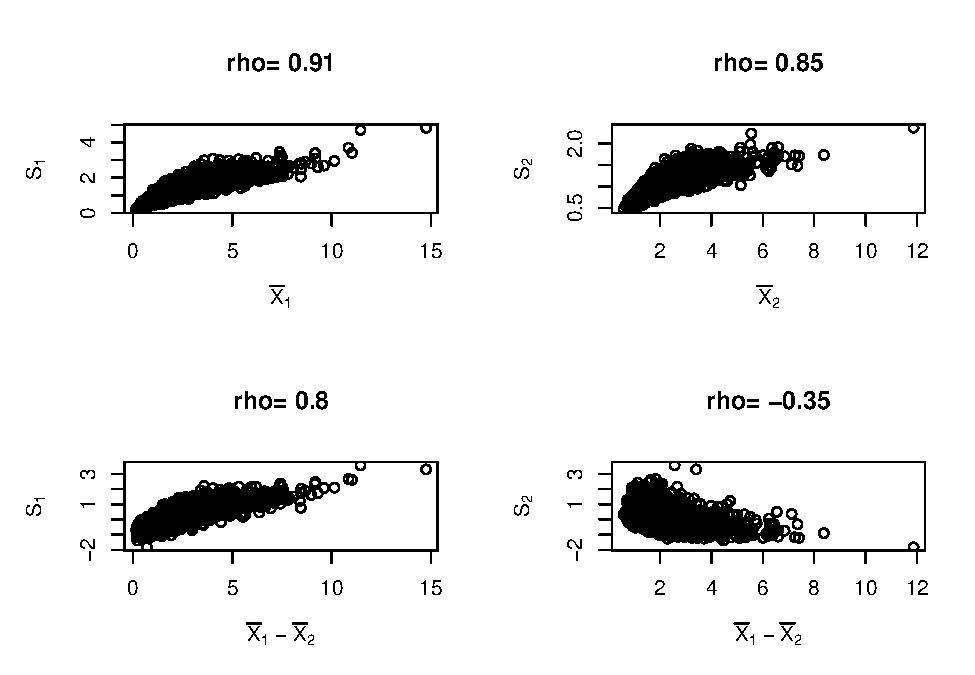
\includegraphics{Correlations-between-the-sample-means-difference-and-standardizers-of-all-estimators,-and-implications-on-biases-and-variances-of-all-estimators_files/figure-latex/SDC2Rs-1.pdf}
\caption{\label{fig:SDC2Rs}\(S_j\) (j=1,2) as a function \(\bar{X_j}\) (top plots) or \(\bar{X_1}-\bar{X_2}\) (bottom plots), when samples are extracted from right skewed distributions (\(\gamma_1 = 6.32\); top plots), with n1=20 and n2=100}
\end{figure}

\begin{figure}
\centering
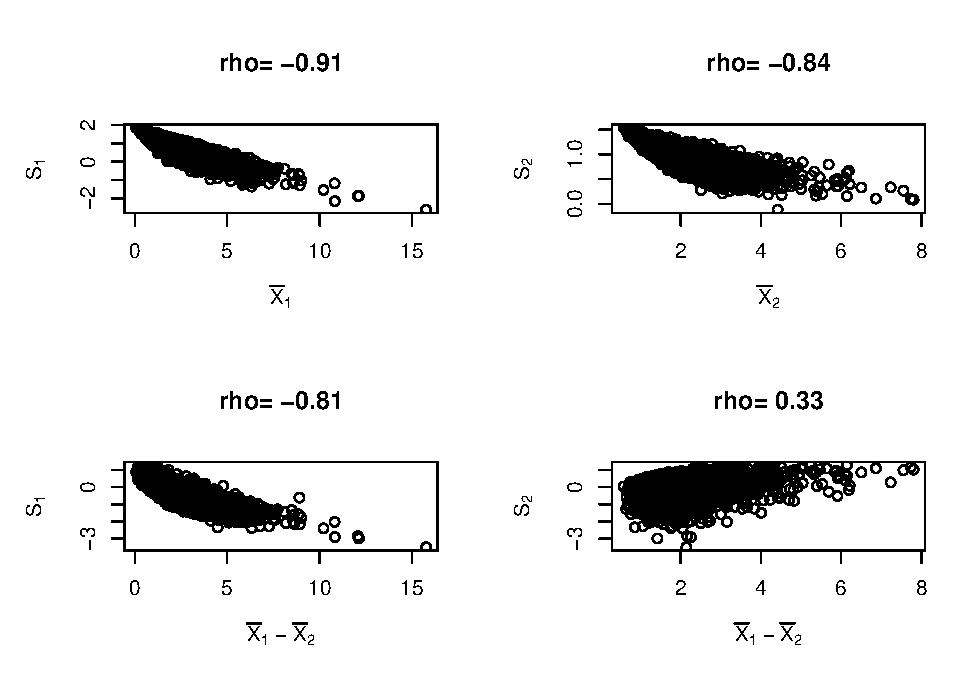
\includegraphics{Correlations-between-the-sample-means-difference-and-standardizers-of-all-estimators,-and-implications-on-biases-and-variances-of-all-estimators_files/figure-latex/SDC2Ls-1.pdf}
\caption{\label{fig:SDC2Ls}\(S_j\) (j=1,2) as a function \(\bar{X_j}\) (top plots) or \(\bar{X_1}-\bar{X_2}\) (bottom plots), when samples are extracted from left skewed distributions (\(\gamma_1 = -6.32\); top plots), with n1=20 and n2=100}
\end{figure}

This might explain why the magnitude of the correlation between \(S_j\) and \(\bar{X_1}-\bar{X_2}\) is lower in the larger sample (See bottom plots in Figures \ref{fig:SDC2Rs} and \ref{fig:SDC2Ls}; note that with no surprise, there is a positive (negative) correlation between \(S_1\) and \(\bar{X_1}-\bar{X_2}\) and a negative (positive) correlation between \(S_2\) and \(\bar{X_1}-\bar{X_2}\) when distribution are right-skewed (left-skewed), as illustrated in the two bottom plots of Figures \ref{fig:SDC2Rs} and \ref{fig:SDC2Ls}).

\begin{figure}
\centering
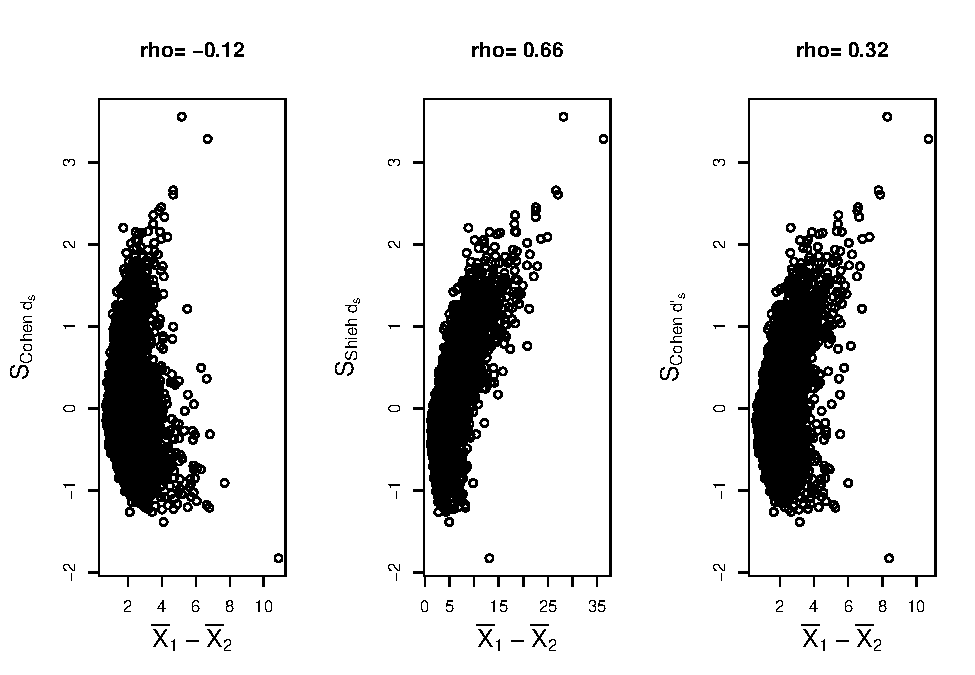
\includegraphics{Correlations-between-the-sample-means-difference-and-standardizers-of-all-estimators,-and-implications-on-biases-and-variances-of-all-estimators_files/figure-latex/StdzrC2Rs-1.pdf}
\caption{\label{fig:StdzrC2Rs}\(S_{Glass's \; d_s}\), \(S_{Shieh's \; d_s}\) and \(S_{Cohen's \; d'_s}\) as a function of the means difference (\(\bar{X_1}-\bar{X_2}\)), when samples are extracted from right skewed distributions (\(\gamma_1 = 6.32\))}
\end{figure}

\begin{figure}
\centering
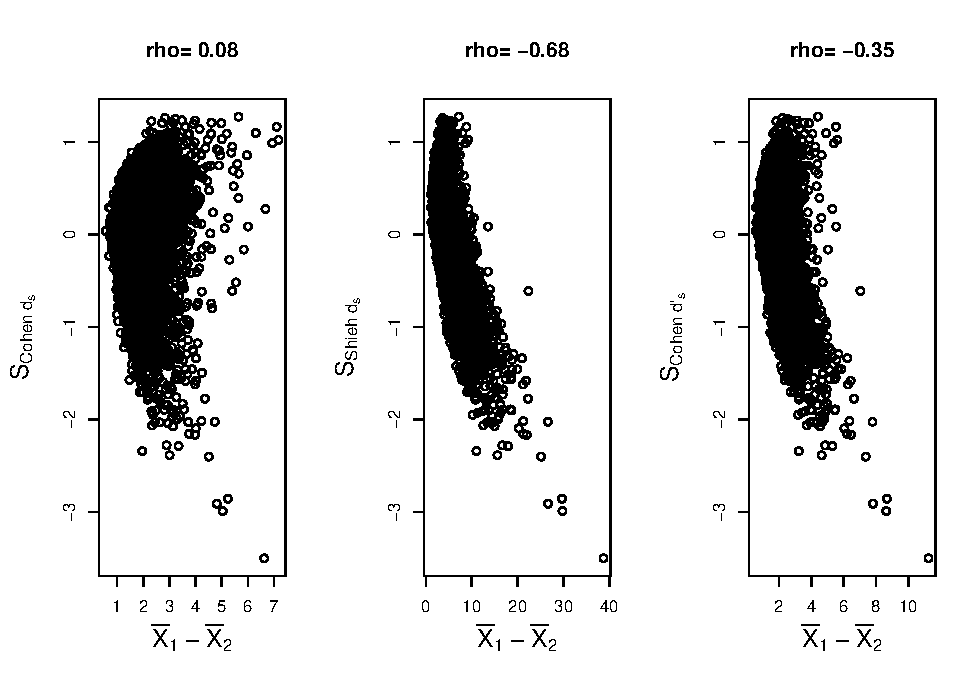
\includegraphics{Correlations-between-the-sample-means-difference-and-standardizers-of-all-estimators,-and-implications-on-biases-and-variances-of-all-estimators_files/figure-latex/StdzrC2Ls-1.pdf}
\caption{\label{fig:StdzrC2Ls}\(S_{Glass's \; d_s}\), \(S_{Shieh's \; d_s}\) and \(S_{Cohen's \; d'_s}\) as a function of the means difference (\(\bar{X_1}-\bar{X_2}\)), when samples are extracted from left skewed distributions (\(\gamma_1 = -6.32\))}
\end{figure}

This might also explain why the standardizers of Shieh's \(d_s\) and Cohen's \(d'_s\) are this time \textbf{correlated} with \(\bar{X_1}-\bar{X_2}\) (see Figures \ref{fig:StdzrC2Rs} and \ref{fig:StdzrC2Ls}):\\
- When computing \(S_{Cohen's \; d'_s}\), the same weight is given to both \(S_1\) and \(S_2\). Therefore, it doesn't seem surprising that the sign of the correlation between \(S_{Cohen's \; d'_s}\) and \(\bar{X_1}-\bar{X_2}\) is the same as the size of the correlation between \(\bar{X_1}-\bar{X_2}\) and the \(SD\) of the smallest sample.\\
- When computing \(S_{Shieh's \; d_s}\), more weight is given to the \(SD\) of the smallest sample, it is therefore not really surprising to observe that the correlation between \(S_{Shieh's \; d_s}\) and \(\bar{X_1}-\bar{X_2}\) is closer of the correlation between \(S_1\) and \(\bar{X_1}-\bar{X_2}\) (i.e.~\(cor(S_{Shieh's \; d_s},\bar{X_1}-\bar{X_2}) > cor(S_{Cohen's \; d'_s},\bar{X_1}-\bar{X_2})\))\\
- When computing \(S_{Cohen}\), more weight is given to the \(SD\) of the largest sample, which by compensation effect, brings the correlation very close to 0.

The correlation \(\bar{X_1}-\bar{X_2}\) and respectively \(SD_1\), \(SD_2\), the standardizer of Hedge's \(g'_s\) and Shieh's \(g_s\) and the standardizer of Hedge's \(g_s\) are summarized in Table 2:

\begin{longtable}[]{@{}lcc@{}}
\caption{Correlation between standardizers (\(SD_1\),\(SD_2\),\(S_{Cohen's \; d_s}\) and others) and \(\bar{X_1}-\bar{X_2}\), when samples are extracted from skewed distributions with equal variances, as a function of the n-ratio.}\tabularnewline
\toprule
& \textbf{\textbf{population distribution}} &\tabularnewline
\midrule
\endfirsthead
\toprule
& \textbf{\textbf{population distribution}} &\tabularnewline
\midrule
\endhead
& \emph{right-skewed} & \emph{left-skewed}\tabularnewline
& ---------------------------------- & -----------------------------------------\tabularnewline
When \(n_1=n_2\) & \(SD_1\): \emph{positive} & \(SD_1\): \emph{negative}\tabularnewline
& \(SD_2\): \emph{negative} & \(SD_2\): \emph{positive}\tabularnewline
& Others: \emph{null} & Others: \emph{null}\tabularnewline
& &\tabularnewline
When \(n_1>n_2\) & \(SD_1\): \emph{positive} & \(SD_1\): \emph{negative}\tabularnewline
& \(SD_2\): \emph{negative} & \(SD_2\): \emph{positive}\tabularnewline
& Others: \emph{negative} & Others: \emph{positive}\tabularnewline
& \(S_{Cohen's \; d_s}\): \emph{null} & \(S_{Cohen's \; d_s}\): \emph{null}\tabularnewline
& &\tabularnewline
When \(n_1<n_2\) & \(SD_1\): \emph{positive} & \(SD_1\): \emph{negative}\tabularnewline
& \(SD_2\): \emph{negative} & \(SD_2\): \emph{positive}\tabularnewline
& Others: \emph{positive} & Others: \emph{negative}\tabularnewline
& \(S_{Cohen's \; d_s}\): \emph{null} & \(S_{Cohen's \; d_s}\): \emph{null}\tabularnewline
\bottomrule
\end{longtable}

\hypertarget{when-unequal-population-variances-are-estimated-based-on-equal-sample-sizes-condition-c}{%
\subsection{When unequal population variances are estimated based on equal sample sizes (condition c)}\label{when-unequal-population-variances-are-estimated-based-on-equal-sample-sizes-condition-c}}

\begin{figure}
\centering
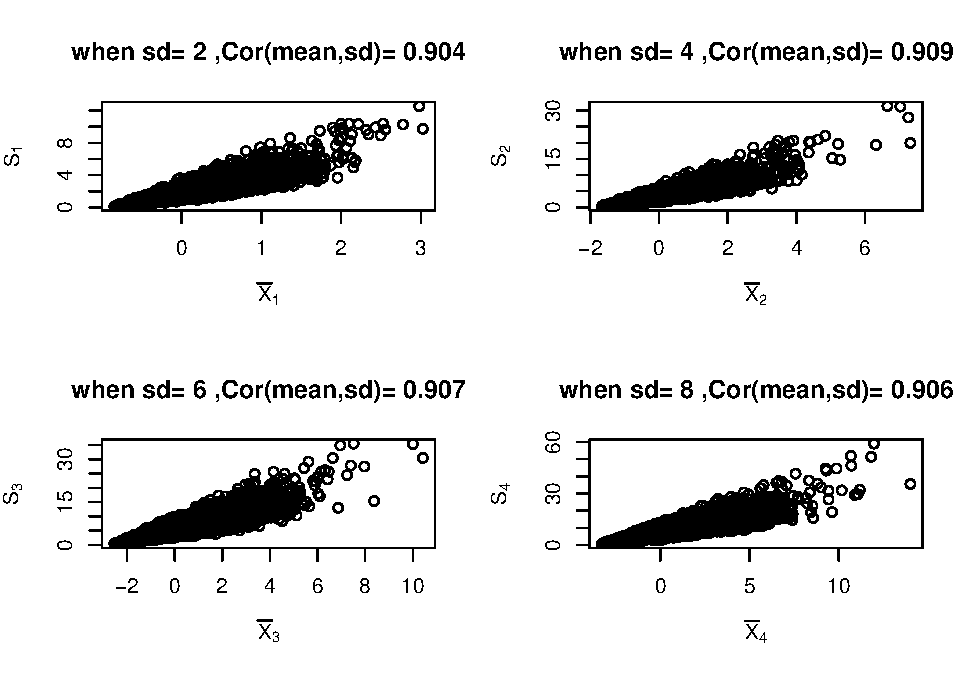
\includegraphics{Correlations-between-the-sample-means-difference-and-standardizers-of-all-estimators,-and-implications-on-biases-and-variances-of-all-estimators_files/figure-latex/C3corn1-1.pdf}
\caption{\label{fig:C3corn1}correlation between \(S_j\) and \(\bar{X_j}\) when n = 25, 50, 75 or 100 and samples are extracted from right skewed distributions (\(\gamma_1 = 6.32\))}
\end{figure}

\begin{figure}
\centering
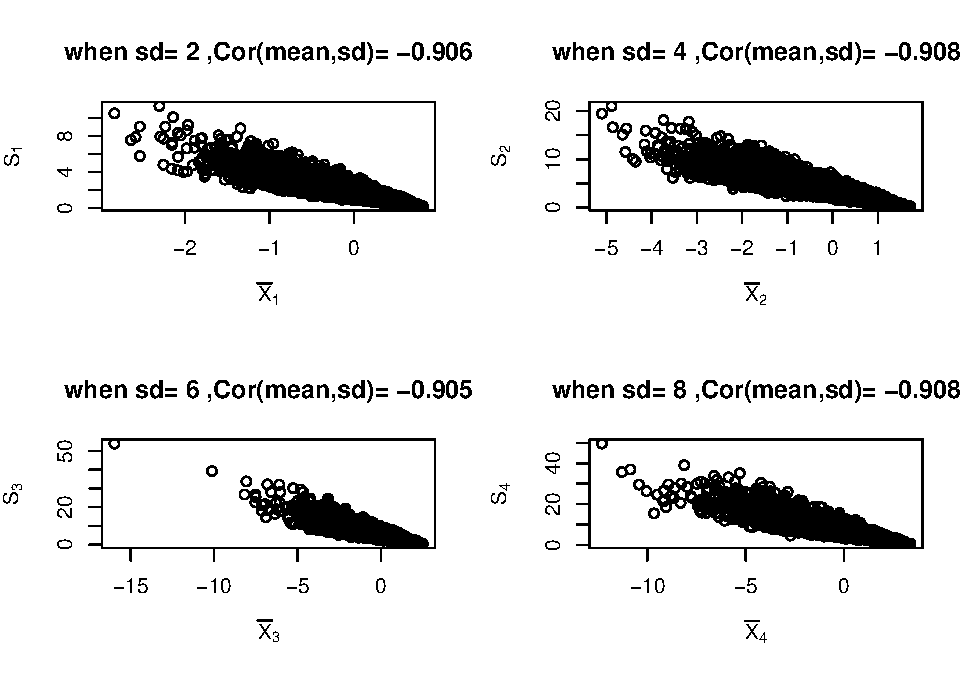
\includegraphics{Correlations-between-the-sample-means-difference-and-standardizers-of-all-estimators,-and-implications-on-biases-and-variances-of-all-estimators_files/figure-latex/C3corn2-1.pdf}
\caption{\label{fig:C3corn2}correlation between \(S_j\) and \(\bar{X_j}\) when n = 25, 50, 75 or 100 and samples are extracted from left skewed distributions (\(\gamma_1 = -6.32\))}
\end{figure}

\begin{figure}
\centering
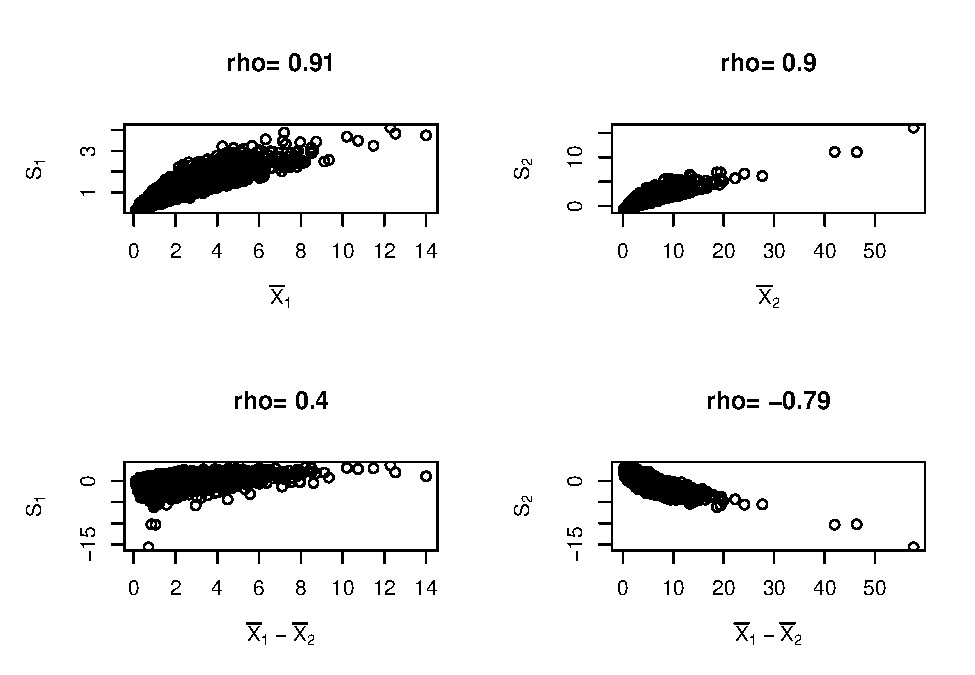
\includegraphics{Correlations-between-the-sample-means-difference-and-standardizers-of-all-estimators,-and-implications-on-biases-and-variances-of-all-estimators_files/figure-latex/SDC3Rs-1.pdf}
\caption{\label{fig:SDC3Rs}\(S_j\) (j=1,2) as a function \(\bar{X_j}\) (top plots) or \(\bar{X_1}-\bar{X_2}\) (bottom plots), when samples are extracted from right skewed distributions (\(\gamma_1 = 6.32\); top plots), with n1=20 and n2=100}
\end{figure}

\begin{figure}
\centering
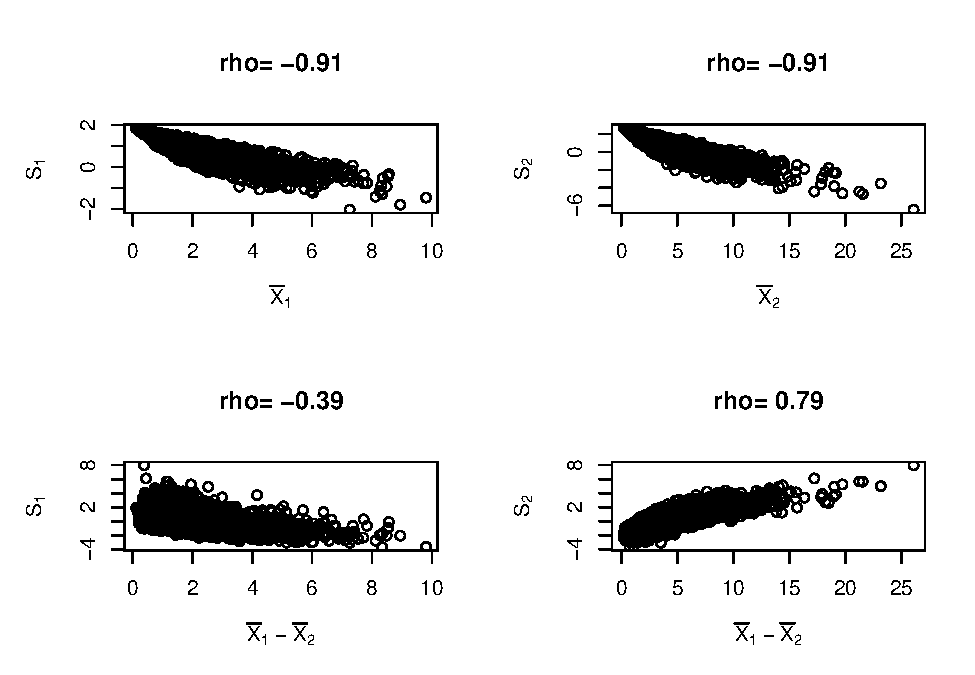
\includegraphics{Correlations-between-the-sample-means-difference-and-standardizers-of-all-estimators,-and-implications-on-biases-and-variances-of-all-estimators_files/figure-latex/SDC3Ls-1.pdf}
\caption{\label{fig:SDC3Ls}\(S_j\) (j=1,2) as a function \(\bar{X_j}\) (top plots) or \(\bar{X_1}-\bar{X_2}\) (bottom plots), when samples are extracted from left skewed distributions (\(\gamma_1 = -6.32\); top plots), with n1=20 and n2=100}
\end{figure}

When distributions are skewed, there are again non-null correlations between \(\bar{X_j}\) and \(S_j\). As illustrated in Figures \ref{fig:C3corn1} and \ref{fig:C3corn2}, the correlation remain the same for any population \(SD\) (\(\sigma\)). However, the magnitude of the correlation between \(S_j\) and \(\bar{X_1}-\bar{X_2}\) differ: it is stronger in the sample extracted from the larger population variance.

\begin{figure}
\centering
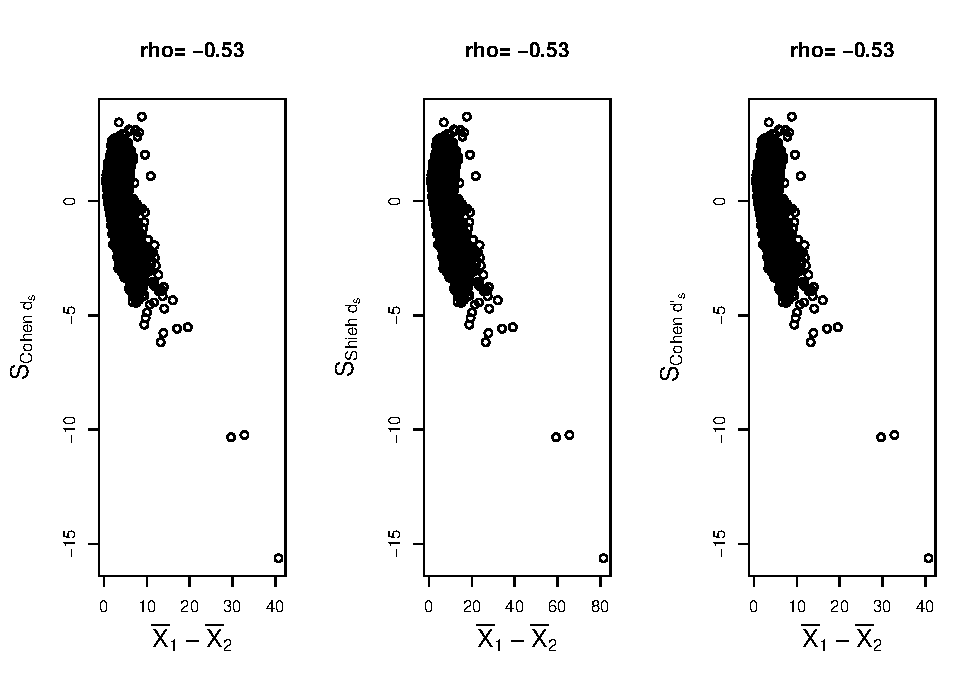
\includegraphics{Correlations-between-the-sample-means-difference-and-standardizers-of-all-estimators,-and-implications-on-biases-and-variances-of-all-estimators_files/figure-latex/StdzrC3Rs-1.pdf}
\caption{\label{fig:StdzrC3Rs}\(S_{Glass's \; d_s}\), \(S_{Shieh's \; d_s}\) and \(S_{Cohen's \; d'_s}\) as a function of the means difference (\(\bar{X_1}-\bar{X_2}\)), when samples are extracted from right skewed distributions (\(\gamma_1 = 6.32\))}
\end{figure}

\begin{figure}
\centering
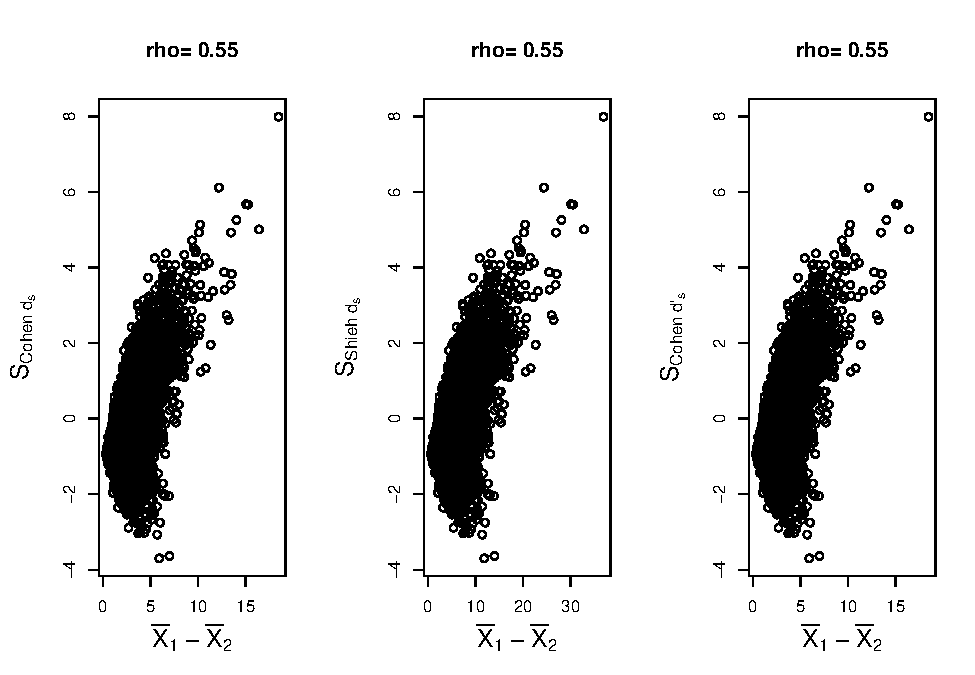
\includegraphics{Correlations-between-the-sample-means-difference-and-standardizers-of-all-estimators,-and-implications-on-biases-and-variances-of-all-estimators_files/figure-latex/StdzrC3Ls-1.pdf}
\caption{\label{fig:StdzrC3Ls}\(S_{Glass's \; d_s}\), \(S_{Shieh's \; d_s}\) and \(S_{Cohen's \; d'_s}\) as a function of the means difference (\(\bar{X_1}-\bar{X_2}\)), when samples are extracted from left skewed distributions (\(\gamma_1 = -6.32\))}
\end{figure}

This also explain that when computing a standardizer taking both \(S_1\) and \(S_2\) into account, it results in a standardizer that is correlated with \(\bar{X_1}-\bar{X_2}\) (see Figures \ref{fig:StdzrC3Rs} and \ref{fig:StdzrC3Ls}). The correlation between the mean difference (\(\bar{X_1}-\bar{X_2}\)) and respectively the standardizer of Shieh's \(d_s\), Cohen's \(d'_s\) and Cohen's \(d_s\) will have the same sign as the correlation between (\(\bar{X_1}-\bar{X_2}\)) and the larger \(SD\). Table 1 summarizes the sign of the correlation between \(\bar{X_1}-\bar{X_2}\) and respectively \(SD_1\), \(SD_2\) and the three standardizers taking both \(SD_1\) and \(SD_2\) into account (see \enquote{Others} in the Table).

\begin{longtable}[]{@{}lcc@{}}
\caption{Correlation between standardizers (\(SD_1\),\(SD_2\) and others) and \(\bar{X_1}-\bar{X_2}\), when samples are extracted from skewed distributions with equal sample sizes, as a function of the SD-ratio.}\tabularnewline
\toprule
& \textbf{\textbf{population distribution}} &\tabularnewline
\midrule
\endfirsthead
\toprule
& \textbf{\textbf{population distribution}} &\tabularnewline
\midrule
\endhead
& \emph{right-skewed} & \emph{left-skewed}\tabularnewline
& --------------------------- & ---------------------------\tabularnewline
When \(\sigma_1=\sigma_2\) & \(SD_1\): \emph{positive} & \(SD_1\): \emph{negative}\tabularnewline
& \(SD_2\): \emph{negative} & \(SD_2\): \emph{positive}\tabularnewline
& Others: \emph{null} & Others: \emph{null}\tabularnewline
& &\tabularnewline
When \(\sigma_1>\sigma_2\) & \(SD_1\): \emph{positive} & \(SD_1\): \emph{negative}\tabularnewline
& \(SD_2\): \emph{negative} & \(SD_2\): \emph{positive}\tabularnewline
& Others: \emph{positive} & Others: \emph{negative}\tabularnewline
& &\tabularnewline
When \(\sigma_1<\sigma_2\) & \(SD_1\): \emph{positive} & \(SD_1\): \emph{negative}\tabularnewline
& \(SD_2\): \emph{negative} & \(SD_2\): \emph{positive}\tabularnewline
& Others: \emph{negative} & Others: \emph{positive}\tabularnewline
& &\tabularnewline
\bottomrule
\end{longtable}

\hypertarget{when-unequal-population-variances-are-estimated-based-on-unequal-sample-sizes-conditions-d-and-e}{%
\subsection{When unequal population variances are estimated based on unequal sample sizes (conditions d and e)}\label{when-unequal-population-variances-are-estimated-based-on-unequal-sample-sizes-conditions-d-and-e}}

\hypertarget{when-distributions-are-right-skewed}{%
\section{When distributions are right-skewed}\label{when-distributions-are-right-skewed}}

We already know that Glass's \(d_s\) using \(SD_1\) will have the smallest bias (and that Glass's \(d_s\) using \(SD_2\) as standardizer will have the largest one) when:\\
- \(n_1 > n_2\) (condition b)\\
- \(\sigma_1 < \sigma_2\) (condition c)
There is therefore no surprises that the most extreme differences between both Glass's estimators (in favour of using \(SD_1\)) occurs when there is a negative pairing between \(n\) and \(SD\), and \(n_1 > n_2\).

\hypertarget{when-distributions-are-left-skewed}{%
\section{When distributions are left-skewed}\label{when-distributions-are-left-skewed}}

We already know that Glass's \(d_s\) using \(SD_2\) will have the smallest bias (and that Glass's \(d_s\) using \(SD_1\) as standardizer will have the largest one) when:\\
- \(n_1 < n_2\) (condition b)\\
- \(\sigma_1 > \sigma_2\) (condition c)
There is therefore no surprises that the most extreme differences between both Glass's estimators (in favour of using \(SD_2\)) occurs when there is a negative pairing between \(n\) and \(SD\), and \(n_1 < n_2\).

\end{document}
